% !TeX spellcheck = en_US
\documentclass[12pt]{article}
\usepackage[utf8]{inputenc}
\usepackage[spanish]{babel}
\usepackage{graphicx}
\usepackage[margin=2.5cm]{geometry}
\usepackage{float}
\usepackage{hyperref}


\usepackage[utf8]{inputenc}
\usepackage{amsmath}
\usepackage{amsfonts}
\usepackage{geometry}
\newcommand{\hrules}{\rule{\linewidth}{0.5mm}}

\begin{document}
	
	\begin{titlepage}
		\centering
		
		\begin{minipage}{0.2\textwidth}
			\begin{flushleft}
				
\includegraphics[width=\textwidth]{logo_ipn.png}
			\end{flushleft}
		\end{minipage}
		\hfill
		\begin{minipage}{0.5\textwidth}
			\centering
			{\scshape\Large Instituto Politécnico Nacional} \\[0.3cm]
			{\scshape\large Escuela Superior de Cómputo}
		\end{minipage}
		\hfill
		\begin{minipage}{0.2\textwidth}
			\begin{flushright}
				
\includegraphics[width=\textwidth]{logo_escom.png}
			\end{flushright}
		\end{minipage}
		
		\vspace{1.5cm}
		
		{\large\textbf{Ingeniería en Inteligencia Artificial}} \\[1.5cm]
		
		{\Large\textbf{Redes Neuronales y Aprendizaje Profundo1}} \\[2cm]
		
		\hrules
		\vspace{0.4cm}
		{\huge\bfseries 
			Práctica 03: Propagación hacía atrás
		} \\[0.4cm]
		\hrules
		\vspace{2.5cm}
		
		% --- INFORMACIÓN PERSONAL ---
		% --- INFORMACIÓN PERSONAL ---
	\begin{minipage}{0.8\textwidth}
		\begin{flushleft} \large
			\textbf{Profesor:} \\
			Saúl de la O Torres 
			\\[1cm]
				Velázquez Arrieta Eduardo Uriel
			\end{flushleft}
		\end{minipage}
		
		\vfill
		
		{\large Fecha de entrega:   2026}
		
	\end{titlepage}
	
	
	\newpage
	\tableofcontents % Índice de contenido
	\vspace{1cm}
	\listoffigures    % Índice de imágenes
	\newpage

\section{Introducción}
El algoritmo de propagación hacia atrás (\textit{backpropagation}) constituye el pilar fundamental para el entrenamiento de redes neuronales artificiales y el desarrollo del aprendizaje profundo moderno. Introducido para superar las limitaciones de los clasificadores lineales como el perceptrón simple, este algoritmo permite calcular de forma analítica y recursiva el gradiente de una función de pérdida respecto a cada uno de los parámetros entrenables (pesos sinápticos y sesgos) a través de la regla de la cadena del cálculo diferencial. Este cálculo sustenta los métodos de optimización basados en gradiente, tales como el Descenso de Gradiente Estocástico (SGD) y sus variantes adaptativas modernas, entre las que destaca Adam (\textit{Adaptive Moment Estimation}).

En la presente práctica se analiza, diseña e implementa el algoritmo de propagación hacia atrás haciendo uso del marco de trabajo \textit{TensorFlow/Keras}, abordando dos vertientes fundamentales del aprendizaje automático:
\begin{enumerate}
	\item \textbf{Procesamiento de Lenguaje Natural (PLN):} Se formula una red neuronal densa precedida por capas de vectorización (\texttt{TextVectorization}) e incrustación de palabras (\texttt{Embedding}) de 16 dimensiones junto con \textit{Global Average Pooling}, orientada al análisis de polaridad y sentimiento en cuatro clases categóricas (\textit{Muy Negativo}, \textit{Neutro}, \textit{Positivo} y \textit{Muy Positivo}).
	\item \textbf{Visión por Computadora con Perceptrón Multicapa (MLP):} Se diseña una arquitectura secuencial profunda densamente conectada compuesta por capas de dimensionalidad $512$, $256$ y $128$ con activaciones ReLU y regularización por \textit{Dropout} ($0.25$), evaluada sobre el conjunto de datos de referencia CIFAR-10 ($60\,000$ imágenes a color de $32\times 32\times 3$ píxeles distribuidas en 10 categorías).
\end{enumerate}

El objetivo central es estudiar el comportamiento de la convergencia de la función de coste (\textit{loss}), la evolución de la métrica de exactitud (\textit{accuracy}) a lo largo de las épocas, y examinar los retos teóricos y prácticos inherentes a los modelos totalmente conectados cuando se enfrentan a entradas de alta dimensionalidad y distribuciones de datos complejos.

\newpage
\section{Desarrollo}

A continuación se detalla la metodología, diseño arquitectónico, implementación y resultados obtenidos para cada una de las actividades programadas en la práctica.

% -----------------------------------------------------------------------------
% ACTIVIDAD 1
% -----------------------------------------------------------------------------
\subsection{Actividad 1: Red Neuronal para Análisis de Sentimiento Multiclase}

Se amplió el problema clásico binario (positivo/negativo) a un esquema de clasificación categórica de cuatro clases, permitiendo capturar gradaciones extremas y niveles de neutralidad:
\begin{itemize}
	\item \textbf{Clase 0 (Muy Negativo):} Manifestaciones de fraude, enojo extremo o pérdida económica total.
	\item \textbf{Clase 1 (Neutro):} Evaluaciones meramente técnicas o informativas sin carga emotiva polarizada.
	\item \textbf{Clase 2 (Positivo):} Conformidad estándar con el producto o servicio recibido.
	\item \textbf{Clase 3 (Muy Positivo):} Expresiones superlativas de satisfacción y recomendación absoluta.
\end{itemize}

\subsubsection{Arquitectura y Preprocesamiento}
El preprocesamiento y extracción de representaciones densas se integró dentro del propio grafo secuencial de TensorFlow/Keras:
\begin{enumerate}
	\item \textbf{Vectorización de Texto (\texttt{TextVectorization}):} Estandarización a minúsculas, remoción de signos de puntuación, delimitación a un vocabulario máximo de $V = 500$ tokens y truncado/relleno fijo a una longitud de secuencia de $L = 12$ tokens.
	\item \textbf{Capa de Incrustación (\texttt{Embedding}):} Proyección del espacio disperso de índices enteros hacia un espacio continuo de $D = 16$ dimensiones.
	\item \textbf{Promedio Global 1D (\texttt{GlobalAveragePooling1D}):} Colapso de la dimensión temporal calculando el vector representativo promedio de la oración.
	\item \textbf{Capas Densas y Regularización:} Dos capas totalmente conectadas con función de activación ReLU ($32$ y $16$ unidades neuronales) acompañadas por un apagado aleatorio (\textit{Dropout}) con tasa de $0.20$ entre ellas.
	\item \textbf{Capa de Salida:} $4$ neuronas con función de activación Softmax para modelar la distribución de probabilidad multiclase:
	\begin{equation}
		P(y = i \mid \mathbf{x}) = \frac{e^{z_i}}{\sum_{j=0}^{3} e^{z_j}}, \quad i \in \{0, 1, 2, 3\}
	\end{equation}
\end{enumerate}

El modelo se optimizó mediante Descenso de Gradiente basado en Adam ($\alpha = 0.005$) minimizando la pérdida de entropía cruzada categórica dispersa (\textit{sparse categorical crossentropy}) a lo largo de 120 épocas de entrenamiento.

\subsubsection{Evaluación Cualitativa ante Muestras no Vistas}
Una vez ajustada la red por propagación hacia atrás, se evaluó su capacidad de inferencia sobre cuatro sentencias sintéticas inéditas. En el Cuadro~\ref{tab:nlp_results} se reportan las predicciones arrojadas por la red.

\begin{table}[H]
	\centering
	\caption{Resultados de inferencia del clasificador de texto ante oraciones de prueba.}
	\label{tab:nlp_results}
	\vspace{0.2cm}
	\begin{tabular}{|p{7.5cm}|c|c|c|}
		\hline
		\textbf{Texto de Entrada} & \textbf{Etiqueta Real} & \textbf{Predicción Red} & \textbf{Confianza} \\ \hline
		\textit{``Pague y nunca enviaron nada son unos rateros''} & Muy Negativo & Positivo (Error) & $49.55\%$ \\ \hline
		\textit{``El articulo llego dentro del plazo esperado sin novedades''} & Neutro & Neutro & $84.83\%$ \\ \hline
		\textit{``Me gusto mucho la compra bastante funcional''} & Positivo & Positivo & $95.57\%$ \\ \hline
		\textit{``Espectacular y fantastico totalmente satisfecho con la calidad''} & Muy Positivo & Positivo & $84.63\%$ \\ \hline
	\end{tabular}
\end{table}

\textbf{Análisis del error de clasificación:} Se observa una asignación incorrecta en la primera oración de prueba, la cual fue catalogada como \textit{Positivo} con una certidumbre marginal del $49.55\%$. Dicha patología se atribuye a que tokens clave que definen la queja (como \textit{``rateros''} o \textit{``pagos''}) no existían en el vocabulario sobre el cual se ejecutó el método \texttt{adapt()}. En consecuencia, la capa de vectorización los mapea al token fuera de vocabulario (\textit{Out-Of-Vocabulary}, OOV indexado en 1), forzando a la red a tomar una decisión basada únicamente en palabras neutras o conectores, exhibiendo el límite de cobertura léxica en arquitecturas sin transfer learning o sin subword tokenization (como BPE).

% -----------------------------------------------------------------------------
% ACTIVIDAD 2 Y 3
% -----------------------------------------------------------------------------
\subsection{Actividades 2 y 3: Implementación de la Clase \texttt{RedBackpropagationCIFAR}}

Para sistematizar el ciclo de vida del clasificador basado en propagación hacia atrás, se encapsuló la lógica funcional en una clase en Python orientada a objetos denominada \texttt{RedBackpropagationCIFAR}. Dicha abstracción cumple con los siguientes requerimientos de diseño:
\begin{itemize}
	\item \textbf{Construcción configurable (\texttt{construir\_modelo}):} Define la topología del Perceptrón Multicapa (MLP) mediante aplanado (\texttt{Flatten}), capas densas con activación ReLU parametrizables en dimensionalidad y factor de regularización por \textit{Dropout}. Compila la red con el optimizador Adam y función de pérdida multiclase.
	\item \textbf{Resumen del modelo (\texttt{resumen}):} Invoca la introspección estructural de Keras mostrando las dimensiones de salida por capa y el conteo analítico de parámetros entrenables.
	\item \textbf{Entrenamiento (\texttt{entrenar}):} Conduce el ciclo de propagación y retropropagación del error registrando el objeto \texttt{History} que almacena las trayectorias de \textit{loss} y \textit{accuracy}.
	\item \textbf{Monitoreo visual (\texttt{graficar\_rendimiento}):} Despliega paneles duales con Matplotlib que contrastan las funciones de coste y precisión para los conjuntos de entrenamiento y prueba por época.
	\item \textbf{Persistencia (\texttt{guardar\_modelo} y \texttt{cargar\_modelo}):} Serializa y recupera desde almacenamiento secundario la topología y los pesos sinápticos óptimos en formato nativo \texttt{.keras}.
	\item \textbf{Inferencia en muestras ajenas (\texttt{predecir\_imagen\_externa}):} Incorpora la biblioteca PIL para abrir imágenes arbitrarias (JPG/PNG), convertirlas a espacio cromático RGB, redimensionarlas espacialmente a $32\times 32$ píxeles, normalizar la intensidad a $[0.0, 1.0]$, y determinar la clase de mayor soporte con la función argmax.
\end{itemize}

El Cuadro~\ref{tab:cifar_summary} describe el balance analítico de parámetros de la arquitectura ejecutada con capas ocultas $[512, 256, 128]$ y \textit{Dropout} al $0.25$.

\begin{table}[H]
	\centering
	\caption{Resumen paramétrico de la arquitectura MLP para CIFAR-10.}
	\label{tab:cifar_summary}
	\vspace{0.2cm}
	\begin{tabular}{|l|l|c|r|}
		\hline
		\textbf{Capa (Tipo)} & \textbf{Forma de Entrada} & \textbf{Forma de Salida} & \textbf{Parámetros} \\ \hline
		\texttt{flatten} & $(32, 32, 3)$ & $(3072)$ & $0$ \\ \hline
		\texttt{dense\_3} (Dense) & $(3072)$ & $(512)$ & $3072 \times 512 + 512 = 1\,573\,376$ \\ \hline
		\texttt{dropout\_1} & $(512)$ & $(512)$ & $0$ \\ \hline
		\texttt{dense\_4} (Dense) & $(512)$ & $(256)$ & $512 \times 256 + 256 = 131\,328$ \\ \hline
		\texttt{dropout\_2} & $(256)$ & $(256)$ & $0$ \\ \hline
		\texttt{dense\_5} (Dense) & $(256)$ & $(128)$ & $256 \times 128 + 128 = 32\,896$ \\ \hline
		\texttt{dropout\_3} & $(128)$ & $(128)$ & $0$ \\ \hline
		\texttt{dense\_6} (Dense) & $(128)$ & $(10)$ & $128 \times 10 + 10 = 1\,290$ \\ \hline
		\hline
		\multicolumn{3}{|l|}{\textbf{Total de parámetros entrenables:}} & \textbf{1,738,890} ($6.63$ MB) \\ \hline
		\multicolumn{3}{|l|}{\textbf{Parámetros no entrenables:}} & \textbf{0} ($0.00$ B) \\ \hline
	\end{tabular}
\end{table}

% -----------------------------------------------------------------------------
% ACTIVIDAD 4 Y 5
% -----------------------------------------------------------------------------
\subsection{Actividades 4 y 5: Exploración de Límites y Reporte de Ejecución sobre CIFAR-10}

El conjunto de datos CIFAR-10 se particionó en $50\,000$ imágenes para entrenamiento y $10\,000$ imágenes para validación/prueba. Las intensidades en el rango $[0, 255]$ se escalaron al intervalo normalizado $[0.0, 1.0]$. Se configuró un tamaño de lote (\textit{batch size}) de $64$ y un horizonte de optimización de $15$ épocas.

\subsubsection{Dinámica de Convergencia del Algoritmo}
A lo largo del entrenamiento, se capturó la evolución de las métricas en cada época. El Cuadro~\ref{tab:training_log} consolida la traza numérica obtenida durante la ejecución.

\begin{table}[H]
	\centering
	\caption{Traza de entrenamiento por propagación hacia atrás sobre CIFAR-10 (15 épocas).}
	\label{tab:training_log}
	\vspace{0.2cm}
	\begin{tabular}{|c|c|c|c|c|}
		\hline
		\textbf{Época} & \textbf{Loss (Train)} & \textbf{Accuracy (Train)} & \textbf{Loss (Val)} & \textbf{Accuracy (Val)} \\ \hline
		1  & $2.0366$ & $24.43\%$ & $1.8465$ & $32.35\%$ \\ \hline
		2  & $1.9000$ & $30.14\%$ & $1.8103$ & $34.96\%$ \\ \hline
		3  & $1.8484$ & $32.24\%$ & $1.7701$ & $37.06\%$ \\ \hline
		4  & $1.8187$ & $33.26\%$ & $1.7162$ & $39.02\%$ \\ \hline
		5  & $1.7971$ & $34.45\%$ & $1.7099$ & $38.33\%$ \\ \hline
		6  & $1.7838$ & $34.99\%$ & $1.6842$ & $39.64\%$ \\ \hline
		7  & $1.7656$ & $35.48\%$ & $1.6744$ & $39.89\%$ \\ \hline
		8  & $1.7543$ & $35.90\%$ & $1.6834$ & $40.50\%$ \\ \hline
		9  & $1.7374$ & $36.51\%$ & $1.6479$ & $41.01\%$ \\ \hline
		10 & $1.7375$ & $36.63\%$ & $1.6374$ & $41.76\%$ \\ \hline
		11 & $1.7247$ & $37.17\%$ & $1.6473$ & $40.65\%$ \\ \hline
		12 & $1.7170$ & $37.64\%$ & $1.6327$ & $\mathbf{42.18\%}$ \\ \hline
		13 & $1.7110$ & $37.62\%$ & $1.6607$ & $41.69\%$ \\ \hline
		14 & $1.7019$ & $38.25\%$ & $\mathbf{1.6050}$ & $42.06\%$ \\ \hline
		15 & $\mathbf{1.6982}$ & $\mathbf{37.97\%}$ & $1.6612$ & $40.44\%$ \\ \hline
	\end{tabular}
\end{table}

\begin{figure}[H]
	\centering
	% Coloca aquí el archivo PNG generado por matplotlib, por ejemplo: curvas_cifar10.png
	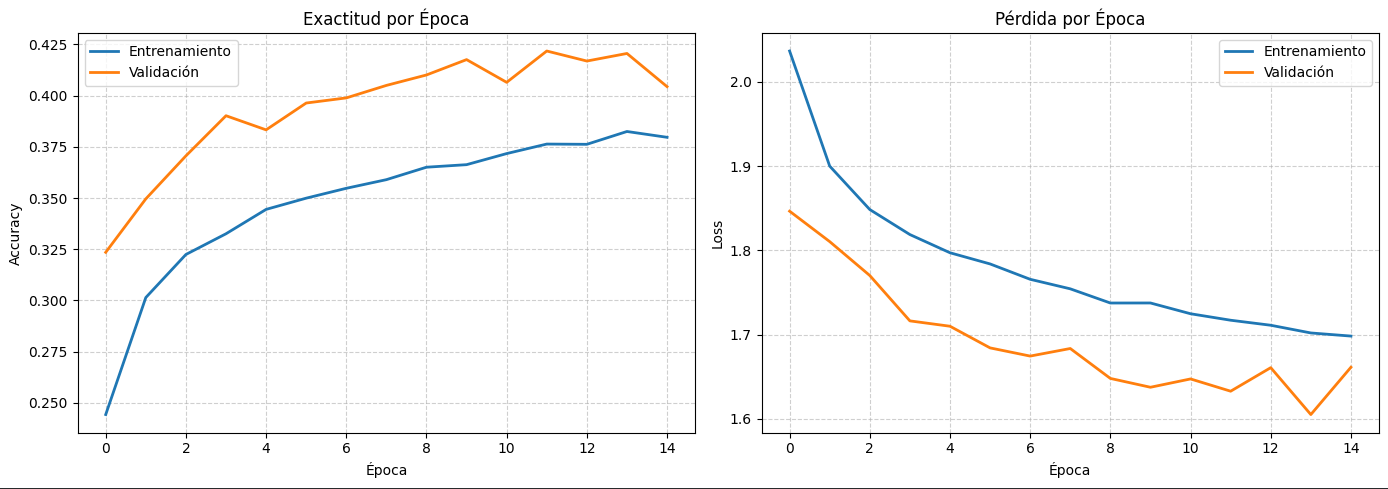
\includegraphics[width=0.92\textwidth]{img1.png}
	\caption{Curvas de convergencia: Exactitud (izquierda) y Función de Pérdida (derecha) en entrenamiento y validación para CIFAR-10.}
	\label{fig:curvas_cifar}
\end{figure}

\subsubsection{Análisis de Límites de la Red Densa vs. Porcentajes de Clase}
En problemas de clasificación balanceada con 10 clases independientes, un clasificador puramente aleatorio (\textit{random guess}) exhibe un límite inferior teórico de precisión del $10.0\%$. 

El modelo implementado por propagación hacia atrás logró superar con holgura dicho umbral basal, alcanzando una cota máxima de validación de:
\begin{equation}
	\text{Accuracy}_{\max}^{\text{val}} = 42.18\% \quad (\text{en la época } 12)
\end{equation}

No obstante, al empujar la red hacia el límite de convergencia con optimizadores de segundo orden implícito como Adam, se constata un estancamiento asintótico temprano alrededor del $42\%$, fenómeno que se fundamenta teóricamente en tres aspectos:
\begin{enumerate}
	\item \textbf{Destrucción de la topología espacial:} Al colapsar la matriz de imagen tridimensional mediante \texttt{Flatten}, cada píxel se procesa como una variable independiente. La red pierde toda noción de vecindad local, bordes, texturas e invariancia ante rotaciones o traslaciones espaciales.
	\item \textbf{Complejidad paramétrica desbalanceada:} Más del $90.4\%$ de los parámetros de la red ($1.57$ millones de $1.73$ millones) radican de forma estricta en la conexión entre la entrada de $3\,072$ dimensiones y la primera capa oculta de $512$ neuronas. Esto ocasiona que el cálculo analítico de gradientes:
	\begin{equation}
		\frac{\partial \mathcal{L}}{\partial \mathbf{W}^{[1]}} = \boldsymbol{\delta}^{[1]} (\mathbf{x})^T
	\end{equation}
	tenga que lidiar con una superficie de optimización no convexa sumamente rugosa y con abundancia de puntos de ensilladura (\textit{saddle points}).
	\item \textbf{Robustez del Dropout:} La tasa de $0.25$ impidió una divergencia catastrófica entre la curva de entrenamiento ($37.97\%$) y la de validación ($40.44\% - 42.18\%$), manteniendo controlada la generalización pero evidenciando que para trascender la barrera del $50\%$ en este corpus se hace mandatorio el reemplazo de transformaciones afines por núcleos de convolución bidimensionales con compartición de pesos (\textit{weight sharing}).
\end{enumerate}

Finalmente, la serialización del modelo concluyó de forma satisfactoria, registrándose en el archivo \texttt{mi\_red\_cifar10.keras} para su posterior reutilización e inferencia sobre imágenes ajenas mediante el método \texttt{predecir\_imagen\_externa()}.
\newpage
\section{Conclusión}
A partir del desarrollo de las arquitecturas y el análisis de las métricas obtenidas durante las fases de entrenamiento y validación, se establecen las siguientes conclusiones:

\begin{itemize}
	\item \textbf{Efectividad del ajuste de gradientes en NLP:} El modelo para análisis de sentimiento demostró la capacidad de la combinación de capas de \textit{Embedding} y capas densas para proyectar un espacio discreto de texto hacia una representación continua donde la propagación hacia atrás optimiza adecuadamente las fronteras de decisión para muestras similares. No obstante, al evaluarse ante oraciones con vocabulario no presente en el corpus de ajuste (como el término coloquial \textit{"rateros"}), el modelo presentó sesgos clasificando incorrectamente una queja severa como sentimiento positivo. Esto pone de manifiesto que el algoritmo de \textit{backpropagation} está estrictamente acotado por la representatividad y cobertura del conjunto de entrenamiento.
	
	\item \textbf{Limitaciones del Perceptrón Multicapa (MLP) ante CIFAR-10:} La red entrenada sobre CIFAR-10 alcanzó una exactitud de validación aproximada del $42.18\%$ y una pérdida en validación estabilizada en torno a $1.60$. Estos resultados evidencian las limitaciones intrínsecas de las redes completamente densas frente a datos espaciales:
	\begin{itemize}
		\item El aplanado vectorial de una imagen de $32\times 32\times 3$ genera $3\,072$ características de entrada, descartando la correlación bidimensional y la invariancia a traslaciones locales.
		\item Dicha arquitectura requirió más de $1.73$ millones de parámetros entrenables concentrados mayoritariamente en la primera capa oculta ($1\,573\,376$ parámetros), lo cual eleva el coste computacional y propicia un estancamiento en mesetas del espacio de pérdida (\textit{plateaus}) a pesar del uso de optimizadores con momentos como Adam.
	\end{itemize}
	
	\item \textbf{Función de la regularización y funciones de activación:} La incorporación de la función no lineal ReLU mitigó el problema del desvanecimiento del gradiente (\textit{vanishing gradient}) durante la retropropagación en las capas intermedias, mientras que la técnica de \textit{Dropout} ($0.25$) controló exitosamente la brecha entre la curva de entrenamiento y la de validación, evitando un sobreajuste (\textit{overfitting}) severo a lo largo de las 15 épocas.
\end{itemize}

En síntesis, se corroboró el funcionamiento analítico y computacional del algoritmo de propagación hacia atrás como mecanismo universal para optimizar representaciones neuronales, remarcando a su vez la necesidad de seleccionar arquitecturas especializadas (tales como redes convolucionales para visión artificial y recurrentes o basadas en atención para lenguaje) en función de la topología de los datos.

\newpage
\section{Referencias}
\begin{enumerate}
	\item Rumelhart, D. E., Hinton, G. E., \& Williams, R. J. (1986). \textit{Learning representations by back-propagating errors}. Nature, 323(6088), 533--536.
	\item Goodfellow, I., Bengio, Y., \& Courville, A. (2016). \textit{Deep Learning}. MIT Press. Recuperado de: \url{http://www.deeplearningbook.org}
	\item Kingma, D. P., \& Ba, J. (2014). \textit{Adam: A method for stochastic optimization}. arXiv preprint arXiv:1412.6980.
	\item Krizhevsky, A. (2009). \textit{Learning multiple layers of features from tiny images}. Technical Report, University of Toronto.
	\item Srivastava, N., Hinton, G., Krizhevsky, A., Sutskever, I., \& Salakhutdinov, R. (2014). \textit{Dropout: a simple way to prevent neural networks from overfitting}. The Journal of Machine Learning Research, 15(1), 1929--1958.
	\item Chollet, F. (2021). \textit{Deep Learning with Python} (2da ed.). Manning Publications.
\end{enumerate}
\end{document}